\section{Behandling}
Behandlingsforløbet for et knæled med artrose har flere komponenter, behandlingen kan både kirurgiske og ikke-kirurgiske alt afhængt af graden af artrose.
\subsection*{Knæledet}
Knæet, \textit{articulatio genus}, er synovialt, sammensat led med en bevægelsesgrad fra 0 til 135$\degree$ fleksion til 0 til 5$\degree$ ekstension. Knæleddet er legemets største led, hvormed det også er udsat for større mekaniske påvirkninger end noget andet led i kroppen. Hermed er knæleddet hyppigere end noget andet led sæde for patologiske forandringer. Knæleddet er sammensat af 3 dele; \textit{femur}, \textit{tibia} og \textit{patella}. Disse er alle i slidfladerne beklædt med et tykt lag hyalinbrusk, op til 7 mm på femur. Sammen med meniskerne, der fordeler trykket på en større overflade, er hyalinbrusken med til at mindske friktionen i leddet. [Bevægeapperatets anatomi]

\begin{figure}[H] 
\begin{center}
\includegraphics[width=0.7\textwidth]{figures/bProblemanalyse/Artose_knae}
\end{center}
\caption{Når det normale knæ undergår patologiskeforandringer ved knæartrose vil strukturne i knæet forandre sig. Brusken kan ved infektion, slid eller traume blive beskadiget, hvilket vil eksponerer knoglen og førere til smerte.\citep{schroder} \citep{adobe}} 
\label{fig:tka_implant} 
\end{figure}

\subsection{Ikke-kiurgisk behandling}

Artrose kan som tidligere nævnt ikke helbredes, men non-kirurgiske behandlingsmetoder vil fortrinsvis søge at smertelindre samt forbedre funktionen \citep{brostrom2012}.En essentiel del af behandling af knæartrose, består af at informere og uddanne patienten, med henblik på at patienten opnår indsigt i sygdommen, samt at patienten aktiv inddrages i behandlingsforløbet .Ved  patientuddannelse forståes også, hvis nødvendig, at opnå et vægttab som kan være med til at reducere belastiningen på det afficerede led \citep{brostrom2012}.
Ved behandling af artrose benyttes også medcin af forskellig karakter til smertelindring samt forbedring af funktionen. De benyttede præperater er først og fremmest Parcetamol som  førstevalgspræperat, men  også NSAID præparaterå kunne være gavnligt ved inflammation \citep{schroder}. Ved kraftige smertegener, hvor anden smertelindrende behandling ikke har haft den ønskede smertelindring, kan opioider også benyttes. Derudover findes andre medikamenter, som for eksempel steroidinjektioner, glucosamin præparater for at nævne nogle få. Derudover benyttes også blandt andet ganghjælpemidler, tapening og skinner. Disse benyttes dog i et mindre omfang \citep{brostrom2012}.\\\\

I behandlingsforløbet for knæartrose er træning, en vigtig faktor, både før og efter en eventuel operationen. Dette afspejler sig også i at der i både nationale og internationale kliniske retninger er bred konsensus om, at træning er af væsentlig betydning ved behandling af  knæartrose  \citep{brostrom2012}.  I et systematisk review , hvor der indgik data fra over 4000 patienter viste at hverken graden af den røntgenpåviste artrose eller smerteintensitet havde indvirkning på hvor stor effekt der kunne forventes af træningsforløbet, altså patienter med svær artrose havde en lige så stor smertereduktion som patienter med let til moderat artrose \citep{Syssorenskou}. 
Smertelindringen der kan forventes ved træning er lige så stor som ved brug af NSAID og større end  ved brug parcetamol, derudover har træning den fordel, at den ikke deler de samme bivirkninger som den smertelindrende medicin \citep{sorenskou}.
I et dansk studie, der strakte sig over 12 måneder blev 100 patienter  der var egnet til at modtage en TKA, randomiseret til modtage modtage enten non-kirurgisk behandling som bestod af et træningsforløb, patientundervisning, indlægssåler og et eventuel vægtabsprogram. Den anden gruppe modtog kirurgisk behandling efterfulgt af et non-invasivt forløb. Gruppen der gennemgik kirurgisk behandling efterfulgt af  et non-invasivt forløb, havde en større smertelindring en gruppen der kun modtog ikke-kirugisk behandling. Dog havde gruppen der modtog kirurgisk behandling større risiko for at få alvorlige komplikationer. Forsøget viste også at over over to tredjedele af gruppen ikke fik foretaget en TKA inden de 12 måneder \citep{newEngland}. Dette kan muligvis betyde at et non-invasivt forløb kan være være med til udskyde et operativt indgreb.

%\subsection{Knæartrose}
%
%Knæartrose også kaldet slidgigt i knæene, har mange årsager. Hvor af nogle er overvægt, arv, traume eller tungt arbejde. Arterose er karakteriseret ved ødelæggelse af ledbrusken med dertil hørende reaktioner i de tillæggende knogler og slimhinder. Symptomerne på knæartrose er smerte, funktionstab og fejlstilling, hvilket besværliggøre hverdagen. 
%Ved knæartrose er sidste behandlings skridt kirurgi, afhængig af graden af traumet er forskellige kirurgiske indgreb en mulighed. [Nationale retningslinjer] 

\subsection{Kirurgisk behandling}

Når de ikke-kirurgiske behandlingsmuligheder har vise en utilstrækkelig effekt er kirurgi det næste skridt i behandlingsforløbet. Der findes flere behandlingsmuligheder inden for kirurgiskbehandling af artrose, hvor af der findes afarter af operationen afhængigt af den enkelte patients situation. Valget af operation og typen af den afhænger af flere faktorer, blandt andet patients alder, aktivitets niveau og hvor fremskreden artrosen er.

\subsubsection{Osteotomi}
Ved degenerative forandringer i knæleddet, grundet primær eller postttrumatisk knæledsarterose, kan patienter opleve belastningsreleaterede smerter, hvilket blandt andet kan skyldes fejlstilling. Osteotomi har tilfomål at afhjælpe den mekaniske belastning i det berørte område, for der ved at afhjælpe smerterne. Ved osteotomi fjernes en kile af knoglen(typisk tibia) og det resterende knogle sikres med skruer og metal plader, proceduren ændre knæets mekaniske akse, hvilket vil ændre belastningen af de degenererede områder.\citep{Osteotomi_og_TKA} Ved yngere(>50-65 år)\citep{Osteotomi_og_TKA} og aktive patienter vil der være større tilbøjlighed til at tilbyde osteotomi frem for den mere invasive TKA, derfor anbefales osteotomi af sundhedstyrelsen til behandling af mildere former for artrose med fejlstilling hos yngre og aktive patienter. [Nationale retningslinjer] Behandlingen ses som en temporær behandling der kan udskyde behovet for TKA, ifølge et Kohordestudie kan der forventes en smertelindring os 80\% af patienterne der får udført osteotomi. (79)(80) I følge [Nationale retningslinjer] må det forventes at 30-50\% af patienterne der får foretatget en osteotomi også vil få behov for en alloplastik operation. [Nationale retningslinjer] Tilbagevenden af smerter korreleres til tab af korrektionen, samt progression af artrosen. Hvorved en TKA kan komme på tale. \citep{Osteotomi_og_TKA} \textbf{Der er data på mere specifikke tilfredsheds undersøgelser, men ser ikke nogen trund til at medtage dem. }

\subsubsection{Alloplastik}
Alloplastik er et operativt indgreb der har til formål helt eller delvist at udskifte knæleddet, med specielt designede metal- og plastkomponenter som varig erstatning for bruskfladerne i knæet. Operationen opdeles i TKA og UKA, hvilket henholdsvis er helt eller delvis udskiftning af knæleddet og afhænger af den specifikke diagnose. Der kan ved traume tilfælde eller svære beskadigelser af de anatomiske strukturer omkring knæet forekomme specialiserede udgaver af knæalloplastik.

\begin{figure}[H] 
\begin{center}
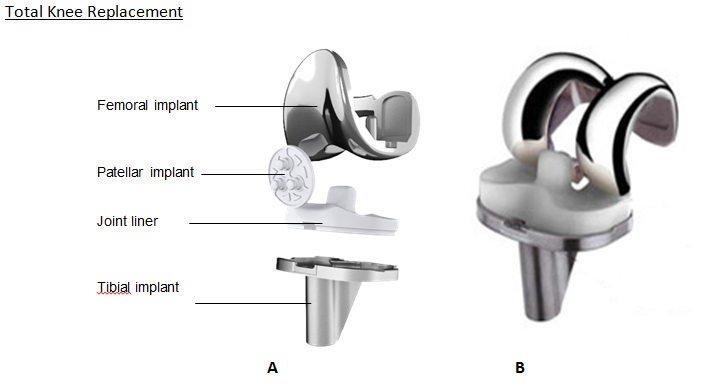
\includegraphics[width=0.7\textwidth]{figures/tka_implant}
\end{center}
\caption{Komponenterne til en total knæalloplastik, består af et femural og tibia implantat ofte bestående af en titaniumlegering. Patella- og tibiaindsatsen er lavet af polyethylen, hvilket er med til at mindske friktionen og efterligne knæledes naturlige bevægelse.\cite{1}} 
\label{fig:tka_implant} 
\end{figure}

Under selve operationen ligger patienten supineret på operationsbordet med knæet i en flekteret position. Et longitudinelt snit lægges over midten af patella. Patella og senerne eleveres og blotter knæleddet, hvilket giver kirurgen adgang til bruskfladerne på femur og tibia. Herefter fjerner kirurgen det ødelagte brusk, ved hjælp af en guideblok der skrues ind i femur og sikrer præcis fjernelse af den ønskede mængde væv. Dette gentages på tibia, hvorved der skabes plads til implantaterne. Midlertidige implantater indsættes for at sikre bevægelsesfriheden er bevaret og testes ved ekstension af knæet for at sikre at den rigtige mænge brusk og knogle materiale er fjernet. Når kirurgen er tilfreds med resultatet bores der guidehuller i henholdsvis femur, tibia og patella til fastemontering af de permanente implantater. Fastmontering sker ved at dække implantatet og monteringsstedet i bencement der limer proteserne fast til den eksisterende knogle struktur. Herefter sikres endnu engang at bevægelsesgraden er bibeholdt, førend indsnittet lukkes og operationen er fuldendt. En TKA operation varer typisk omkring én time, hvorefter patienten kan støtte på benet den følgende dag. Efter operationen følger et rehabiliteringsforløb for at støtte og styrke muskulaturen omkring knæet.\citep{Sanna2013} \citep{tka-technique}

I følge sundhedsstyrelsens vurdering er knæalloplastik, som behandling af knæartrose, effektiv til at mindske smerte, øge funktion og derved bedre livskvalitet.[Nationale retningslinjer] Holdbarheden af knæimplantaterne vurderes ud fra antallet af implantater der er blevet udskiftet efter 10 år, hvor det findes at 90 til 95\% af implantaterne ikke er revideret. Dog skal nævnes at det ikke er muligt at vurdere holdbarheden af den enkelte protese, da flertallet af patienter dør med en velfungerende implantat. [Nationale retningslinjer]

\paragraph{Succeskriterier}

Succeskriterier for kirurgisk behandlingen af arterose er ifølge styrringsgruppen for Dansk knæalloplastikregister (DKA) \citep{aarsrapport2016} opdelt i fem kriterier, som alle bygger revisionsraten. Altså patienter som har behov for en yderligere knæ operation.  

% Please add the following required packages to your document preamble:
% \usepackage{graphicx}
% \usepackage[table,xcdraw]{xcolor}
% If you use beamer only pass "xcolor=table" option, i.e. \documentclass[xcolor=table]{beamer}
\begin{table}[H]
\centering
\caption{Tabellen viser succeskriterierne for knæalloplastikoperationer med en standard acceptabel grænse sammenholdt med landsgennemsnittet. Spredning er indikeret i parentes. Tabellen er modificeret fra \citep{aarsrapport2016} }
\label{succeskriterier}
\resizebox{\textwidth}{!}{%
\begin{tabular}{lcc}
\hline
\rowcolor[HTML]{C0C0C0} 
Indikator                                                                                                                                                                                                                                                  & Standard    & \begin{tabular}[c]{@{}c@{}}Landsgennemsnit\\ (Spredning)\end{tabular} \\ \hline
\begin{tabular}[c]{@{}l@{}}\textbf{Genindlæggelse}\\ \\ Andel af alle patienter med primær knæalloplastik på baggrund af primær artrose, \\ der genindlægges uanset diagnose indenfor 30 dage efter udskrivning\end{tabular}                                        & Højest 10\% & 7,3 \% (5,8-9,5)                                                      \\ \\
\begin{tabular}[c]{@{}l@{}}\textbf{Revisionsrate det første postoperative år}\\ \\ Andel af alle patienter med primær knæalloplastik fra et givent operationsår, \\ der er revideret (dvs. implantat fjernes, udskiftes eller tilføjes) indenfor 1 år.\end{tabular} & Højest 3\%  & 1,8 \% (0,8-2,4)                                                      \\ \\
\begin{tabular}[c]{@{}l@{}}\textbf{Revisionsrate de første 2 postoperative år}\\ \\ Andel af alle patienter med primær knæalloplastik fra et givent operationsår, \\ der er revideret (dvs. implantat fjernes eller udskiftes) indenfor 2 år.\end{tabular}          & Højest 5\%  & 3.3\% (1,7-4,8)                                                       \\ \\
\begin{tabular}[c]{@{}l@{}}\textbf{Revisionsrate de første 5 postoperative år}\\ \\ Andel af alle patienter med primær knæalloplastik fra et givent operationsår, \\ der er revideret (dvs. implantat fjernes, udskiftes eller tilføjes) indenfor 5 år.\end{tabular}   & Højest 8\%  & 6,0\% (4,2-6,7)                                                       \\ \\
\begin{tabular}[c]{@{}l@{}}\textbf{Mortalitet indenfor 90 dage}\\ \\ Andel af patienter, der dør indenfor 90 dage efter primær knæalloplastik.\end{tabular}                                                                                                         & Højest 1\%  & 0,4\% (0,0-0,7)                                                      
\end{tabular}%
}
\end{table}

Fra \tabref{succeskriterier} ses det at der fra et organisatorisk synspunkt er overholdt de succeskriterier som er opstillet fra styringsgruppens side. Sammenlignet med patient tilfredsheden er der dog en skævhed. Hvor utilfredsheden fra patienterne ligger på 11-25\% Dette kan tyde på at der er et problem i forbindelse med knæoperationen , operationen forløber efter retningslinjerne og har lave revisionsrater men patienterne er stadig utilfredse, hvor op mod 39\% oplevede moderat til alvorlig smerte. \citep{aarsrapport2016} \citep{Bourne2010} \citep{Sakellariou2016}

\textbf{Overgang til smerte afsnit.}
%
%(1) http://www.robodoc.com/patient_about_faqs.html
%
%(2) https://www.youtube.com/watch?v=tKji04oFGdU

% (3) http://www.ortopaedi.dk/fileadmin/Guidelines/Referenceprogrammer/Osteotomi_og_TKA.pdf

	%(4) Surgical approaches in total knee arthroplasty.
	
%	(5) tka-technique
%
%(79) Dahl AW, Toksvig-Larsen S, Roos EM. A 2-year prospective study of patient- relevant outcomes in patients operated on for knee osteoarthritis with tibial osteot- omy. BMC Musculoskeletal Disorders 2005;6(1):18. Er lagt på mendlay
%(80) Hoell S, Suttmoeller J, Stoll V, Fuchs S, Gosheger G. The high tibial osteoto- my, open versus closed wedge, a comparison of methods in 108 patients. Arch Or- thop Trauma Surg 2005;125(9):638-643. Er lagt på mendelay